capture program drop doreg
program doreg, eclass
	syntax varlist(min=2 fv) [if] [in] [, fe(varlist fv) dist(real 500) comp(varlist) tag(string)] 
	token `varlist' // tokenize list of passed variables for use
	local and = "&" // default is to add extra condition to passed if statement
	if "`if'"=="" { // if the "if" passed is blank, then
		local and = "if" // include the "if" explicitly
	}

	capture drop res_*
	capture drop int_*
	qui areg `1' `if' `and' inlist(`comp',0,1), absorb(`fe') // demean the productivity variable over passed FE variable
		// do this only if it matches passed "if" statement
		// do this only if it has a valid 0/1 value in the group variable
	local df_fe = e(df_a) // save off degrees of freedom from absorbing FE for use in adjusting SE later
	
	capture drop res_`1'
	qui predict res_`1', res // create residuals of productivity variable
	
	qui areg `2' `if' `and' inlist(`comp',0,1), absorb(`fe') // demean the rural density variable over passed FE variable
	capture drop res_rurd
	qui predict res_rurd, res // create residual of density variable
	capture drop int_rurd
	qui gen int_rurd = res_rurd*`comp' // create interaction of residual density and comparison group variable
	
	local i = 3 
	while "``i''" != "" { // for all the remaining controls
		qui areg ``i'' `if' `and' inlist(`comp',0,1), absorb(`fe') // demean the control over passed FE variable
		capture drop res_cntl_``i''
		qui predict res_cntl_``i'', res // create residual of control variable
		capture drop int_cntl_``i''
		qui gen int_cntl_``i'' = res_cntl_``i''*`comp' // create interaction of residual control with comparison group variable
		local ++i
	}

	// Main results
	// Regress productivity on density, include all controls, include all interaction terms, and a constant(c), 
	qui ols_spatial_HAC res_`1' res_rurd int_rurd res_cntl_* int_cntl_* `comp' c `if' `and' inlist(`comp',0,1), ///
			lat(y_cent) lon(x_cent) timevar(c) panelvar(c) distcutoff(`dist') lagcutoff(1)	// options for spatial errors
	//qui reg res_`1' res_rurd int_rurd res_cntl_* int_cntl_* `comp' `if' `and' inlist(`comp',0,1) // OLS version for testing, leave commented out
	qui tabulate name_0 `if' `and' e(sample)==1 & `comp'==0 // count countries in group=0
	qui estadd scalar N_country = r(r) // store country count for group=0
	qui count `if' `and' e(sample)==1 & `comp'==0 // count observations in group=0
	qui estadd scalar N_obs = r(N) // store obs count for group=0
	local df_adj = e(df_r)/(e(df_r)-`df_fe') // Df adjustment for estimated FE
	mat NV = `df_adj'*e(V) // adjust all C/V matrix
	
	ereturn repost V = NV
	qui estadd scalar p_zero = 2*(1-t(e(df_r),abs(_b[res_rurd])/_se[res_rurd])) // add p-value for H0: beta=0 for group==0		
	qui estadd scalar p_diff = 2*(1-t(e(df_r),abs(_b[int_rurd])/_se[int_rurd])) // add p-value for H0: beta(group=0) = beta(group=1)
	estimates store `tag'2 // store results

	qui lincom res_rurd + int_rurd // get linear combination of base and interaction to get estimated elasticity, SE for group==1	
	local comp_se = r(se) // save off the SE of this estimate
	
	// Run separate OLS for reference group, for reporting use
	// To avoid running spatial OLS again, pull the appropriate SE from the prior spatial OLS
	// Done solely to avoid re-running spatial OLS again to save time
	qui reg res_`1' res_rurd res_cntl_* `if' `and' `comp'==1 // run regression on just the comparison group ==1, the reference
	mat NV = e(V) // save OLS Var/Covar matrix
	mat NV[1,1] = `comp_se'^2 // overwrite Var/Covar for density with the variance from spatial OLS above
	ereturn repost V = NV // repost the overwritten Var/Covar to estimates for reporting
	qui tabulate name_0 `if' `and' e(sample)==1 & `comp'==1 // count countries in group=1
	qui estadd scalar N_country = r(r) // store country count for group=1
	qui count `if' `and' e(sample)==1 & `comp'==1 // count observations in group=1	
	qui estadd scalar N_obs = r(N) // store obs count for group=1
	qui estadd scalar p_zero = 2*(1-t(e(df_r),abs(_b[res_rurd])/`comp_se'))
	estimates store `tag'1 // store results
	
	label variable res_rurd "Log labor/land ratio ($\beta_g$)"


end 

//////////////////////////////////////////////////////////////////////////////////////////////////////////
// Supplemental program to run spatial interaction regression
// - Variables are all demeaned first to save time
// - Spatial OLS for a single group based on if statement (MUST have if statement)
/////////////////////////////////////////////////////////////////////////////////////////////////////////
capture program drop onereg
program onereg, eclass
	syntax varlist(min=2) [if] [in] [, fe(varlist) dist(real 500) tag(string)] 
	token `varlist' // tokenize list of passed variables for use
		
	qui areg `1' `if', absorb(`fe') // demean the productivity variable over passed FE variable
	capture drop res_`1'
	qui predict res_`1', res // create residuals of productivity variable
	
	qui areg `2' `if', absorb(`fe') // demean the rural density variable over passed FE variable
	capture drop res_rurd
	qui predict res_rurd, res // create residual of density variable
	
	local i = 3 
	while "``i''" != "" { // for all the remaining controls
		qui areg ``i'' `if', absorb(`fe') // demean the control over passed FE variable
		capture drop res_cntl_``i''
		qui predict res_cntl_``i'', res // create residual of control variable
		local ++i
	}

	// Regress productivity on density, include all controls, and a constant(c), 
	qui ols_spatial_HAC res_`1' res_rurd res_cntl_*  c `if', ///
			lat(y_cent) lon(x_cent) timevar(c) panelvar(c) distcutoff(`dist') lagcutoff(1)	// options for spatial errors
	qui tabulate name_0 `if' & e(sample)==1 // count countries in group=0
	qui estadd scalar N_country = r(r) // store country count for group=0
	qui count `if' & e(sample)==1 // count observations in group=0
	qui estadd scalar N_obs = r(N) // store obs count for group=0
	qui estadd scalar p_zero = 2*(1-t(e(df_r),abs(_b[res_rurd])/_se[res_rurd])) // add p-value for H0: beta=0 for group==0		
	estimates store `tag'1 // store results
	
	label variable res_rurd "Log labor/land ratio ($\beta_g$)"

end 

//////////////////////////////////////////////////////////////////////////////////////////////////////////
// Supplemental program to run spatial interaction regression with three groups
// - Variables are all demeaned first to save time
/////////////////////////////////////////////////////////////////////////////////////////////////////////
capture program drop threereg
program threereg, eclass
	syntax varlist(min=2) [if] [in] [, fe(varlist) dist(real 500) comp(varlist) tag(string)] 
	token `varlist' // tokenize list of passed variables for use
	
	local and = "&" // default is to add extra condition to passed if statement
	if "`if'"=="" { // if the "if" passed is blank, then
		local and = "if" // include the "if" explicitly
	}

	capture drop res_*
	capture drop int_*

	qui areg `1' `if' `and' inlist(`comp',0,1,2), absorb(`fe') // demean the productivity variable over passed FE variable
		// do this only if it matches passed "if" statement
		// do this only if it has a valid 0/1 value in the group variable
	local df_fe = e(df_a) // save off degrees of freedom from absorbing FE for use in adjusting SE later
	capture drop res_`1'
	qui predict res_`1', res // create residuals of productivity variable
	
	capture drop comp1
	capture drop comp2
	qui gen comp1 = (`comp'==1) // create separate dummy for 1st comp category
	qui gen comp2 = (`comp'==2) // create separate dummy for 2nd comp category
	
	qui areg `2' `if' `and' inlist(`comp',0,1,2), absorb(`fe') // demean the rural density variable over passed FE variable
	capture drop res_rurd
	qui predict res_rurd, res // create residual of density variable
	capture drop int_rurd_1
	capture drop int_rurd_2
	qui gen int_rurd_1 = res_rurd*comp1 // create interaction of residual density and comparison group variable
	qui gen int_rurd_2 = res_rurd*comp2 // create interaction of residual density and comparison group variable
		
	local i = 3 
	while "``i''" != "" { // for all the remaining controls
		qui areg ``i'' `if' `and' inlist(`comp',0,1,2), absorb(`fe') // demean the control over passed FE variable
		capture drop res_cntl_``i''
		qui predict res_cntl_``i'', res // create residual of control variable
		capture drop int_cntl_``i''_1
		capture drop int_cntl_``i''_2
		qui gen int_cntl_``i''_1 = res_cntl_``i''*comp1 // create interaction of residual control with comparison group variable
		qui gen int_cntl_``i''_2 = res_cntl_``i''*comp2 // create interaction of residual control with comparison group variable
		local ++i
	}

	// Main results
	// Regress productivity on density, include all controls, include all interaction terms, and a constant(c), 
	qui ols_spatial_HAC res_`1' res_rurd int_rurd_* res_cntl_* int_cntl_* comp1 comp2 c `if' `and' inlist(`comp',0,1,2), ///
			lat(y_cent) lon(x_cent) timevar(c) panelvar(c) distcutoff(`dist') lagcutoff(1)	// options for spatial errors
	//reg res_`1' res_rurd int_rurd_* res_cntl_* int_cntl_* comp1 comp2 `if' `and' inlist(`comp',0,1,2) // OLS version for testing, leave commented out
	qui tabulate name_0 `if' `and' e(sample)==1 & `comp'==0 // count countries in group=0
	qui estadd scalar N_country = r(r) // store country count for group=0
	qui count `if' `and' e(sample)==1 & `comp'==0 // count observations in group=0
	qui estadd scalar N_obs = r(N) // store obs count for group=0
	local df_adj = e(df_r)/(e(df_r)-`df_fe') // Df adjustment for estimated FE
	mat NV = `df_adj'*e(V) // adjust all C/V matrix
	ereturn repost V = NV
	qui estadd scalar p_zero = 2*(1-t(e(df_r),abs(_b[res_rurd])/_se[res_rurd])) // add p-value for H0: beta=0 for group==0		
	qui estadd scalar p_diff1 = 2*(1-t(e(df_r),abs(_b[int_rurd_1])/_se[int_rurd_1])) // add p-value for H0: beta(group=0) = beta(group=1)
	qui estadd scalar p_diff2 = 2*(1-t(e(df_r),abs(_b[int_rurd_2])/_se[int_rurd_2])) // add p-value for H0: beta(group=0) = beta(group=1)
	estimates store `tag'1 // store results
	
	label variable res_rurd "Log labor/land ratio ($\beta_g$)"


end 


To support the idea that the GAEZ-derived measures of TFP are related to actual TFP in a log-linear manner, we rely on the evidence presented by Galor and Ozak in the supplemental material to their 2016 paper. They show the relationship of their GAEZ-derived measure (which we mimic to a great extent) to actual production measures (harvested amounts), suggesting that the GAEZ measure is picking up a significant fraction of actual production across pixels (in their case). This isn't a strict test of the log-linearity assumption, but provides some assurance that the GAEZ measure picks up real differences in production.
\subsection{Migration between districts}
The prior scenario requires the use of controls for non-agricultural productivity and the capital/labor ratio because we assume that there is no movement of factors across districts, and that therefore the wage and rental rate are district-specific. A different scenario involves the assumption that factors are, in fact, mobile across districts within a given state (although no assumption is necessary about migration across states).

If factors are mobile across districts, and the returns are thus equalized, then 
then for agriculture it must be that $w_{Ais} = w_{As}$ and $r_{Ais} = r_{As}$. This is again consistent with \citet{young2013inequality} and \citet{hklm2017}, and with the evidence shown in the following section that the pervasive evidence of movement between urban and rural areas implies movement across districts, as most districts in our data are almost entirely rural, or contain only very small villages and towns. Note that this assumption does not imply that the agricultural returns to factors are undistorted, or equal to what we would expect in a competitive equilibrium. It only assumes that all districts in the state face a similar wage and rental rate.

In addition, we still assume that goods are free to move between districts, and thus that $p_{Ais} = p_{As}$ for districts within a state. With these two assumptions in place, we can go back to equation (\ref{EQ_minimizing}), take logs, and re-arrange to
\begin{equation*}
	\ln A_{Ais} = \alpha + \beta \ln L_{Ais}/X_{is} + \ln p_{As} + \phi(1-\beta)\ln r_{As} + \left[1-\phi(1-\beta)\right] \ln w_{As}.
\end{equation*}
Here, the problem of estimating $\beta$ from the relationship of (log) agricultural productivity and the (log) agricultural labor/land ratio becomes straightforward. The price, $p_{As}$, rental rate, $p_{As}$, and wage, $w_{As}$, can all be held constant by including state-level fixed effects in a regression. We do not need to specify how those prices or returns to factors are determined within the state to do this.



Using this capital/labor ratio together with the first-order condition for labor from \ref{EQ_factorprices} and the production function from (\ref{EQ_production}), the cost-minimizing labor/land ratio will satisfy 
\begin{equation}
	\left(\frac{L_{Ais}}{X_{is}}\right)^{\beta} = (1-\beta) p_{Ais} A_{Ais} \left(\frac{\phi}{r_{Ais}}\right)^{\phi(1-\beta)}\left(\frac{(1-\phi)}{w_{Ais}}\right)^{1 - \phi(1-\beta)}. \label{EQ_minimizing}
\end{equation}
As would be expected, this ratio depends positively on productivity, $A_{Ais}$, such that for given output and factor prices, the district will employ more labor per unit of land if they are more productive. Similarly, for a given productivity level and output price, higher wages and/or rental rates for capital will be associated with a lower labor/land ratio.

Without proceeding any further in terms of solving for the actual allocation of workers into the agricultural sector, we can use equation (\ref{EQ_minimizing}) to illustrate the idea behind our estimation strategy. The relationship between the agricultural labor/land ratio, $L_{Ais}/X_{is}$, and agricultural productivity, $A_{Ais}$, is governed by the parameter $\beta$. Taking logs of (\ref{EQ_minimizing}) and re-arranging terms, we have
\begin{equation*}
	\ln A_{Ais} = \alpha + \beta \ln L_{Ais}/X_{is} + \ln p_{Ais} + \phi(1-\beta)\ln r_{Ais} + \left[1-\phi(1-\beta)\right] \ln w_{Ais}
\end{equation*}
where $\alpha$ captures fixed terms involving $\beta$ and $\phi$.\footnote{Formally, $\alpha = -\phi(1-\beta)\ln \phi - \left[1-\phi(1-\beta)\right]\ln (1-\phi) - \ln (1-\beta)$} Holding constant the wage, rental rate, and agricultural price across districts, we could in theory recover an estimate of $\beta$ by from the relationship of (log) agricultural productivity and (log) agricultural labor/land ratio. 

Of course, the central empirical question is whether, in fact, there are conditions under which wages, rental rates, and prices are constant across districts, or if not, whether there are ways to control for them. 



In the following two sub-sections we show how assumptions regarding the mobility of factors and goods between non-agriculture and agriculture within districts, and the mobility of factors between agricultural sectors in different districts, establish conditions under which we can identify $\beta$. Once we lay those out, in the following section of the paper we show the evidence supporting the assumptions regarding mobility that lay behind that identification.

\subsection{Non-agricultural mobility}
To continue, consider the non-agricultural sector. It will have first-order conditions
\begin{eqnarray*}
    w_{Nis} &=& (1-\phi)\frac{Y_{Nis}}{L_{Nis}} \\ 
    r_{Nis} &=& \phi \frac{Y_{Nis}}{K_{Nis}},
\end{eqnarray*}
which will result in a capital/labor ratio of
\begin{equation*}
	\frac{K_{Nis}}{L_{Nis}} = \frac{\phi}{1-\phi} \frac{w_{Nis}}{r_{Nis}}.
\end{equation*}

Here we introduce the first assumption about the mobility of factors. Let labor and capital move freely between the agricultural and non-agricultural sectors \textit{within} a district, such that the returns to capital and labor are equalized across the sectors. This is consistent with recent evidence by \citet{young2013inequality} and \citet{hklm2017}, which we review in more detail in the next section of the paper. This assumption implies that $w_{Ais} = w_{Nis}$ and $r_{Ais} = r_{Nis}$.\footnote{The evidence cited on worker mobility finds that wages appear to be equalized for workers of similar skill levels, although there is heterogeneity in those skills, and hence in total earnings. As written, the model assumes all workers are identical in human capital. We can allow for a difference between skilled/unskilled workers, and for the agricultural sector and non-agricultural sector to differ in the intensity with which those types of workers are used, and it does not alter the conclusions of this sub-section. See the appendix for a demonstration of this.}

With equal wages and rental rates, it will be the case that the capital/labor ratio in both sectors is equal to the district level capital/labor ratio, or $K_{Ais}/L_{Ais} = K_{Nis}/L_{Nis} = K_{is}/L_{is}$. Using that along with the first-order conditions for labor in both sectors, and the production function in (\ref{EQ_production}) and (\ref{EQ_nonag}), we can solve for
\begin{equation}
	\left(\frac{L_{Ais}}{X_{is}}\right)^{\beta} = (1-\beta) \frac{p_{Ais} A_{Ais}}{A_{Nis}} \left(\frac{K_{is}}{L_{is}} \right)^{-\phi\beta}. \label{EQ_laxdistrict}
\end{equation}
This indicates that the agricultural labor/land ratio depends on the relative productivity of agricultural compared to non-agriculture ($A_{Ais}/A_{Nis}$), and the size of the capital/labor ratio at the district level. 

The second assumption is that goods (both agricultural and non-agricultural) are free to move \textit{across} districts within a given state/province. We will make the case in the following section that this is plausible given the small size of individual districts. This assumption implies that the relative price of agricultural goods in a district is equal to the state-level relative price, of $p_{Ais} = p_{As}$. While we are assuming that the relative price is equalized across districts, we are not assuming that the relative price is necessarily undistorted. That is, there may be taxes, subsidies, or other frictions that prevent $p_{As}$ from being equal to a competitive equilibrium price. All that we assume here is that this relative price is common to all the districts within a given state/province. 

With that assumption in hand, we can take logs of the relationship in (\ref{EQ_laxdistrict}) and re-arrange to the following
\begin{equation}
	\ln A_{Ais} = \alpha + \beta \ln L_{Ais}/X_{is} + \ln p_{As} + \ln A_{Nis} + \phi\beta \ln K_{is}/L_{is},
\end{equation}
where now $\alpha = - \ln (1-\beta)$. We could again recover an estimate of $\beta$ by using the relationship of (log) agricultural productivity, $A_{Ais}$, and the (log) agricultural labor/land ratio, $L_{Ais}/X_{is}$. This requires us to hold constant the relative price of agriculture, but that can be accommodated in a regression setting with a state fixed effect, as the term is common to all districts within state $s$. 

We also have to hold constant the non-agricultural productivity level and the district-level capital/labor ratio. To do this, we can introduce controls. In particular, we have data on district-level night lights to proxy for the capital/labor ratio at the district level, as well as the non-agricultural productivity level (described in detail below). In addition, the percent urban in the district is a proxy for both non-agricultural productivity and the capital/labor ratio in this setting, as the percent urban will be a positive function of non-agricultural productivity and the capital/labor ratio. Total population (or urban population) of a district can also be included as a control, allowing for the idea of agglomeration effects influencing the level of productivity in the non-agricultural sector.


\subsection{Theoretical setting}
Consider a district $i$ located in province (or state) $s$. Let the aggregate agricultural production function for that district be given by
\begin{equation}
Y_{Ais} = A_{Ais} X_{is}^{\beta} \left(K_{Ais}^{\phi}L_{Ais}^{1-\phi}\right)^{1-\beta} \label{EQ_production}
\end{equation}
where $A_{Ais}$ is total factor productivity, $X_{is}$ is land, $K_{Ais}$ is capital (or any other inputs aside from land and labor), and $L_{Ais}$ is the number of agricultural workers. The land elasticity we are interested in is $\beta$.\footnote{While we have written the function here as Cobb-Douglas, this is solely for ease of exposition. The analysis does not require this. In the Appendix we show that one could use a general constant returns to scale function to derive a similar estimation equation.}

We assume that operators in this district are cost-minimizers, and take the real wage of agricultural workers and real rental rate of agricultural capital as given. The real wage is denoted by $(1+\tau^w_{is})w_{As}$, where $w_{As}$ is the province average wage, and $(1+\tau^w_{is})$ is a district-specific wedge relative to that average wage, similar to the structure used in \cite{hsieh2009misallocation}. For capital, the real rental rate is $(1+\tau^r_{is})r_{As}$, where $r_{As}$ is the province average rental rate, and $(1+\tau^r_{is})$ is a district-specific wedge on that rental rate. These wedges capture any arbitrary distortion, and not just explicit taxes or subsidies set by governments.

Given the real wage and rental rate, the first-order conditions governing the choice of labor and capital to employ are
\begin{eqnarray}
    (1+\tau^w_{is})w_{As} &=& (1-\phi)(1-\beta) \frac{Y_{Ais}}{L_{Ais}} \\ \nonumber 
    (1+\tau^r_{is})r_{As} &=& \phi(1-\beta)\frac{Y_{Ais}}{K_{Ais}}. \label{EQ_factorprices}
\end{eqnarray}
Given these two conditions, the capital/labor ratio used in the district will be
\begin{equation}
	\frac{K_{Ais}}{L_{Ais}} = \frac{\phi}{1-\phi} \frac{(1+\tau^w_{is})}{(1+\tau^r_{is})} \frac{w_{As}}{r_{As}}. \nonumber
\end{equation}
Using this capital/labor ratio together with the first-order condition for labor from (2) and the production function from (\ref{EQ_production}), the cost-minimizing labor/land ratio will satisfy 
\begin{equation}
	\left(\frac{L_{Ais}}{X_{is}}\right)^{\beta} = (1-\beta) A_{Ais} \left(\frac{\phi}{(1+\tau^r_{is})r_{As}}\right)^{\phi(1-\beta)}\left(\frac{(1-\phi)}{(1+\tau^w_{is})w_{As}}\right)^{1 - \phi(1-\beta)}. \label{EQ_minimizing}
\end{equation}
As would be expected, this ratio depends positively on productivity, $A_{Ais}$, such that for given output and factor prices, the district will employ more labor per unit of land if they are more productive. Similarly, for a given productivity level and output price, higher real wages and/or rental rates for capital will be associated with a lower labor/land ratio.

This relationship forms the basis for our estimation of $\beta$. To make this more clear, take logs of both sides of (\ref{EQ_minimizing}), and re-arrange to the following
\begin{equation}
	\ln A_{Ais} = \alpha + \beta \ln L_{Ais}/X_{is} + \tau_{is} + \omega_s, \label{EQ_est}
\end{equation}
where $\alpha$ is a collection of fixed parameters.\footnote{Formally, $\alpha = -\phi(1-\beta)\ln \phi/(1-\phi) - \ln (1-\phi) - \ln (1-\beta)$}. The last two terms are defined as:
\begin{eqnarray}
	\tau_{is} &=& \phi(1-\beta) \ln (1+\tau^r_{is}) + [1-\phi(1-\beta)] \ln (1+\tau^w_{is}) \\
	\omega_s &=& \phi(1-\beta) \ln r_{As} + [1-\phi(1-\beta)] \ln w_{As}.
\end{eqnarray}
The first term, $\tau_{is}$, is a combined wedge term representing how district $i$ real wages and rental rates deviate from the province averages. The second term, $\omega_s$, captures that province average level of real wages and rental rates. No assumption is necessary about how those province-level rates are set. They may be arbitrarily distorted relative to competitive market equilibrium rates due to taxes, subsidies, barriers to movement of labor and/or capital between provinces, or other frictions. The wedge term $\tau_{is}$ reflects specific policies or distortions (e.g. taxes or subsidies) at the district level. 

The non-agricultural sector is not explicit, but is embedded in the terms involving wages and rental rates. Non-agricultural productivity, taxes, subsidies, or other distortions would, in equilibrium, be reflected in the real rental and wages rates in agriculture. Province-level effects of the non-agricultural sector common to all districts are captured by $\omega_s$. District-specific effects of non-agriculture that create deviations from the province wages or rental rates are picked up by the wedge term $\tau_{is}$.

\subsection{Empirical approach}
Equation (\ref{EQ_est}) shows, in principle, that we could use variation in $A_{Ais}$ and $L_{Ais}/X_{is}$ to estimate the value of $\beta$ using district level data. The province level of average wages and rental rates, $\omega_s$, can be accounted for by fixed effects. Given those province fixed effects, we can identify $\beta$ by looking at the relationship of $\ln A_{Ais}$ to $L_{Ais}/X_{is}$ across districts \textit{within} a given province. This means that the overall \textit{level} of agricultural productivity or rural density at the province level is not used. Therefore distortions to the price of agricultural goods at the province level, wedges between provinces in the real wage or rental rate, or differences in non-agricultural productivity between provinces may all be present in reality, but do not affect our estimation of $\beta$. In particular, differences across provinces (and countries) in the overall level of development (and hence the level of real wages or the real return to capital) do not influence our estimates.

However, the district-specific wedge, $\tau_{is}$, is unobservable. Thus if there is meaningful variation in the real wage or real rental rate of capital across districts \textit{within} a given province, our estimates of $\beta$ may be biased. We cannot measure these wedges directly, and instead use a set of proxy variables to capture their variation. In practice, we replace the wedge terms in equation (\ref{EQ_est}) with $\delta_{\tau}' \mathbf{Z}_{is}$, so that we have
\begin{equation}
	\ln A_{Ais} = \alpha + \beta \ln L_{Ais}/X_{is} + \delta_{\tau}' \mathbf{Z}_{is} + \omega_s, \label{EQ_Omega}
\end{equation}
where $\delta_{\tau}'$ is the vector of coefficients on the controls contained in $\mathbf{Z}_{is}$. We discuss the specific controls included at the end of this section.

Prior to that, a second issue with using equation (\ref{EQ_Omega}) to estimate $\beta$ is the measurement of $A_{Ais}$. We address this by using an agro-climatic measure of inherent productivity. In particular, let overall agricultural productivity be defined by 
\begin{equation}
	\ln A_{Ais} = \ln A_{Ais}^{Agro} + \rho_s + \delta_{A}' \mathbf{Z}_{is}. \label{EQ_prod}
\end{equation}
The first factor is potential agro-climatic productivity, $\ln A_{Ais}^{Agro}$, which captures productivity coming from things such as temperature, rainfall, and soil conditions. This agro-climatic productivity measure is specific to a district. Second, $\rho_s$ captures technological (or institutional or cultural) factors that affect agricultural productivity, common to all districts within a given province $s$. Finally, $\mathbf{Z}_{is}$ captures district-specific observable characteristics that may also influence productivity in agriculture. The term $\delta_{A}'$ is a vector of the effect these characteristics have on productivity, which is distinct from the effect they may have on the wedge term through $\delta_{\tau}'$.

We will measure the agro-climatic productivity term within a district using the work of \cite{galorozak2016}, which is itself built on the Global Agro-ecological Zone project from the \cite{gaez}. We describe the details of the GAEZ data below, but consider it to be a noisy measure of true agro-climatic productivity,
\begin{equation}
	\ln A_{Ais}^{GAEZ} = \ln A_{Ais}^{Agro} + \epsilon_{is}. \label{EQ_gaez}
\end{equation}
Here $\epsilon_{is}$ is a noise term and is assumed to be uncorrelated with true agro-climatic productivity. In short, we assume that the GAEZ did not make systematic errors in measuring agro-climatic productivity. Assessing that will be part of our robustness checks.

Combining (\ref{EQ_gaez}) with (\ref{EQ_prod}), (\ref{EQ_Omega}), and (\ref{EQ_est}) we arrive at a final specification
\begin{equation}
	\ln A^{GAEZ}_{Ais} = \alpha + \beta \ln L_{Ais}/X_{is} + \gamma_{s} + \delta' \mathbf{Z}_{is} + \epsilon_{is}. \label{EQ_regress}
\end{equation}
Here, $\gamma_s = \omega_s + \rho_s$ is a province-specific fixed effect which absorbs the province-level differences in real factor prices and the level of agricultural productivity. The vector $\delta' = \delta_{\tau}' + \delta_{A}'$ is the combined effect of the controls in $\mathbf{Z}_{is}$ on factor prices and productivity.

The specification in (\ref{EQ_regress}) will deliver unbiased estimates of $\beta$ so long as our controls and fixed effects ensure that within-province variation in rural density is not related to $\epsilon_{is}$. To the extent that $\epsilon_{is}$ captures simple GAEZ measurement error in inherent productivity, this should not be problematic. However, more worrisome is the possibility of some systematic district-level variation in wedges or agricultural productivity that is related to rural density. We do not have a natural experiment to leverage for random or quasi-random variation in productivity or rural density that would rule this out. We argue instead that the province fixed effects and controls contained in $\mathbf{Z}_{is}$ capture all the relevant variation in district real factor price wedges and unobserved productivity. 

A reason to believe that the district-specific wedges are not very relevant (even if province- or country- level ones may be) is that each district tends to be quite small relative to its province. The median province has 28 disticts, and the median district contains only 6.7\% of total province population and 7.7\% of total province rural population. In absolute terms, the median district contains only about 26,000 total people, and about 12,500 rural residents. The districts in our dataset are not large relative to the wider economy around them, and as such the province-level fixed effects should capture almost all of the relevant variation in real wages, rental rates, and productivity. As part of our robustness checks, we also exclude particular districts from our sample that \textit{are} large in population, or contain urban areas with more than 25,000 residents, as these may be more likely to have significant district-level wedges to factor prices. We also examine only provinces with more than 50 districts, to ensure we are looking at districts that are relatively small with respect to their province.

Beyond that, we have the sets of controls contained in $\mathbf{Z}_{is}$. To summarize, we include measures of district (log) night light density, the district share of population in urban areas, and the (log) total district population. Among many possible relationships in the data, high night light density and large urban share (relative to the province as a whole) can indicate that real wages or rental rates are higher than in surrounding districts, suggesting positive wedges on those two factor prices. A large population (relative to province as a whole) could imply either a positive or negative wedge on factor prices, depending on if agglomeration or congestion effects prevail. We also include polynomials of all three control variables in a robustness check to allow for non-linear relationships between them, wedges, and unmeasured productivity. For a sub-sample of our main data, we also include controls for demographics and household asset data from the Demographic and Health Surveys to provide more proxies for real wages and rental rates. As we show below, the patterns we find for the elasticity $\beta$ are consistent regardless of the controls we include.


/Users/dietz/Dropbox/GrowthBlog/GrowthEcon/_posts/2016-01-30-Persistence-Technology.md
pandoc https://emanuelfontelles.github.io/cv/ -f html-native_divs -o cv.pdf --pdf-engine=xelatex
pandoc -f html -o deep-roots-2.pdf http://growthecon.com/blog/Deep-Roots-2/ -o deep-roots-2.pdf

pandoc -o ~/Dropbox/GrowthBlog/PostPDF/test.pdf 2019-01-11-Deep-Roots-2.md --template=/Users/dietz/dropbox/tools/latex.template

pandoc -o "~/dropbox/work/2019-01-11-Deep-Roots-2.pdf" "/Users/dietz/Dropbox/GrowthBlog/GrowthEcon/_site/blog/Deep-Roots-2/index.html" "--template=/Users/dietz/dropbox/tools/latex.template"

/Users/dietz/Dropbox/GrowthBlog/GrowthEcon/_site/blog/Deep-Roots-2/index.html

### Explaining divergence
If you take a standard growth course, then none of this makes sense. There is no way the gap should get *wider* over time. Why? Well, any initial differences in the stocks of inputs like physical or human capital should dissipate over time as countries with less of them have faster growth of these inputs than countries with more of them. Even if you expand yourself to theories of endogenous growth through the accumulation of ideas, the mechanics all suggest that places which start behind should eventually catch up - or at least should not fall behind further. Ideas can be copied, and trailing countries have a bigger stock of ideas to copy from, whereas leaders have to keep coming up with new things. 

The speed at which a country should converge to the steady state in any of these modern growth models is fast enough that at the time scales we are looking at (1820 to 2010) any initial gaps should have long ago disappeared. It took Germany and Japan, at most, five decades to catch up to the U.S. after World War II. The countries at the bottom of the distribution in the figures above have had two *centuries* to catch up, and have not. So it is almost surely not slow convergence speeds that are the culprit here.

If it isn't slow convergence, then what does a modern growth model tell us is the reason for the disparity in living standards? Exogenous parameters, like the savings rate or the level of total factor productivity. But if it is exogenous parameters, then the model itself doesn't offer us anything in terms of explanation. Which isn't to dismiss the Solow model or endogenous growth theory out of hand. They have a place in explaining many features of modern growth. To the extent that they are useful here, it is in putting a name on which underlying exogenous parameters we should be looking at. Although "the level of total factor productivity" is hardly a beacon of clarity. 

The point is that digging more deeply into the origins of savings behavior (e.g. how patient are people in a given country?) or the willingness to adopt new technologies (e.g. how open to change are people?) or other fundamental parameters is not some tangent in understanding growth. It is *central* to understanding why some countries are rich and others poor. 




\begin{table}[!htb]
\begin{center}
\caption{Number of districts by Temperate/Tropical status}
\label{TAB_breakdown}
{\small
\begin{tabular}{llccr}
\midrule
& & \multicolumn{2}{c}{Suitable for:} & \\ \cmidrule(lr){3-4}
& & Tropical & Temperate & Number of\\
& Sample & Crops    & Crops     & Districts \\ \midrule
1. & Excluded & No & No & 10 \\
2. & Tropical sample & Yes & No & 9,088 \\
3. & Temperate sample & No  & Yes & 10,661 \\
4. & Excluded & Yes & Yes & 15,692 \\ \midrule
   & Total    &     &     & 35,451 \\
\midrule
\end{tabular}
}
\end{center}
\vspace{-.5cm}\singlespacing {\footnotesize \textbf{Notes}: The table shows the number of districts included in the two major sub-samples used in our analysis, the ``temperate'' and ``tropical''. These are defined by their suitability for specific crops. Tropical crops are cassava, cowpeas, pearl millet, sweet potatoes, wet rice, and yams. Temperate crops are barley, buckwheat, rye, oats, white potato, and wheat. ``Excluded'' groups are not used in the analysis.
}
\end{table}


Combining this constraint with a positive relationship of living standards and population growth yields the canonical Malthusian model of stagnation  The importance of this ``Malthusian constraint'' in production can be measured by the elasticity of output with respect to land. Much of the literature, while acknowledging land is necessary, does not concern itself with the specific size of this elasticity, nor consider the possibility that the elasticity may vary across economies. In this paper, we first establish that the quantitative effect of productivity and population on living standards depends on the size of this elasticity. Then, in the main contribution of the paper, we provide estimates of the elasticity across different geographic and political regions. These estimates show significant variation, with a larger elasticity - a ``tighter'' Malthusian constraint - in temperate areas and a smaller elasticity in tropical areas. This in turn implies that living standards are more sensitive to population and productivity shocks in temperate areas, with consequences for subsequent development. 

To establish the importance of the elasticity of agricultural output with respect to land - the ``land elasticity'' hereafter - we provide a static two-sector model of agriculture and non-agriculture with several key features. First, we consider an economy that is made up of many locations, each with its own stock of agricultural land, but where labor and other inputs move freely between locations. This reveals a simple cross-sectional relationship between the density of agricultural workers in a location and agricultural total factor productivity (TFP) that provides us with a specification we can use to estimate the land elasticity. Second, we allow for the presence of factors beyond land and labor (e.g. capital), and show that our estimation strategy does not rely on data on these other inputs. Last, by incorporating an explicit non-agricultural sector and using non-Gorman preferences over agriculture and non-agriculture that allows for non-homotheticity \citep{boppart2014} we are able to derive simple analytical solutions for real income per capita and the share of labor in agriculture. This shows that the elasticity of both outcomes with respect to population and productivity (in either sector) is increasing with the land elasticity. As agriculture becomes more sensitive to the use of land, living standards and the agricultural labor share both become more sensitive to shocks. The intuition is that as agricultural output becomes more sensitive to land, it becomes \textit{less} sensitive to capital and labor, and hence it takes larger movements of those inputs into or out of agriculture to reach equilibrium in response to a change in population or productivity. The implication is that areas with a high land elasticity develop faster in response to positive productivity shocks or drops in population, but also suffer more from population increases and negative productivity shocks.

Theoretically, variation in the land elasticity across economies could be important in explaining comparative development. But does the land elasticity vary at all? To answer that we estimate the land elasticity for different samples of districts (i.e. 2nd level administrative units) from around the world. As noted, our basic specification is taken from the production side of our model, which shows that under mild assumptions the spatial distribution of \textit{agricultural} workers across districts \textit{within} provinces or states is informative about the land elasticity in those districts. Province-level fixed effects capture unobservable information on non-labor inputs, and we do not rely on cross-country comparisons, nor do we have to assume the land elasticity is homogenous within countries. 

All of our estimates come from within-province variation. It is important to note that our specification is derived from only the agricultural production side of our model. The assumptions we made regarding preferences and non-agricultural production are used solely to illustrate the importance of the land elasticity for living standards, and are not relevant for the empirical work.



Further, we are estimating the aggregate production function elasticity for land, and the underlying farm-level production functions that give rise to the factor share data may not share the same elasticity. For agricultural production, this has been discussed since \citet{Hayami:1970ly}, and is an application of \citet{houthakker1955}, where an aggregate Cobb-Douglas may represent the envelope of a set of different techniques, each of which may have an elasticity of substitution between factors different than one (including zero). The factor share information, assuming markets are complete, may provide an accurate estimate of the elasticity of output with respect to land conditional on a fixed technique, but the aggregate elasticity we estimate can differ given the possibility of changing techniques. 


\vspace{.5cm}\noindent\textbf{Measurement Error in rural density:} If there were classical measurement error in rural density, then our estimated $\beta_g$ would be subject to attenuation bias. If one believes the variance of the measurement error is \textit{larger} in tropical areas, such as South-east Asia or tropical Africa, then the estimated elasticity will be attenuated more than in temperate areas, and this could explain the pattern of results we have found. 

The most likely source of this on the population side would seem to be poor census-taking procedures in the countries in tropical regions. We cannot rule this out, but the scale of the measurement error necessary to account for the differences appears extreme. For example, we estimate that $\beta_g$ is almost 0.25 for temperate districts, and approximately 0.125 for tropical districts. For this two-fold difference to have been driven by measurement error in the tropical region, the true variance in (log) rural density would have to be \textit{half} of the measured variance. This in turn would imply that half of the rural densities from HYDE were overstated by a factor of two or more, or understated by a factor of one-half or less. It seems implausible that measurement error in rural density could be this dramatic, and moreover only this dramatic in tropical countries.

More worrisome would be some kind of systematic measurement error in rural density. Given our empirical setting, this would have to be systematic measurement error across districts \textit{within} provinces. And further, the systematic measurement error would have to be present predominantly in either tropical or temperate regions, but not both, in order to account for the results. For example, if within tropical provinces it was the case that relatively dense districts had their density over-reported (and less dense districts had their density under-reported) then it would appear that the correlation of density to agricultural productivity was very large, and hence $\beta_g$ would be estimated to be very small. We cannot rule this out (or the logical opposite of systematic smoothing of rural density counts within temperate provinces), but it is not obvious why such systematic errors would take place \textit{within} provinces but only for one type of climate area. It is not a question of development level, as we are not comparing relatively rich temperate areas to relatively poor tropical areas, but are rather comparing districts within provinces to one another. 

The underlying HYDE data on district-level rural populations is taken from administrative data, not an imputation. As noted above in the robustness sub-section, IPUMS data confirms that the rural data is a strong proxy for agricultural workers, so it is unlikely to be that in tropical areas our rural density is overstating agricultural density in some districts versus others. Also, as mentioned earlier, we can eliminate any district that has a medium-sized urban area located within it, which might perhaps lead to overstatesment of rural density, and our results hold.

\subsection{Results by Political Regions}
Based on the patterns of elasticities seen by crop suitability and climate zone, we would expect that land constraints vary across groups of countries within specific political regions (e.g. Northwest Europe or Southeast Asia). Here we show significant differences in the estimated $\beta_g$ when we group districts by these political regions. In these classifications, we will be forcing all districts within a nation to belong to the same geographic region, and hence have a common $\beta_g$. This obscures variation in agro-climatic conditions within nations. Nevertheless, it is interesting to see how the values of $\beta_g$ vary across political regions, as so much other research on economic development is based on these kinds of regional distinctions, rather than at the agro-climatic level.

Table \ref{TAB_beta_subregion} shows the estimates for fifteen separate regions, the exact definitions of which can be found in the Appendix. We start in Panel A, column (1) with North and Western Europe. The estimated value is 0.259, consistent with column (2), where the estimated value for Eastern Europe is 0.287, and column (3) where the estimated value for Southern Europe is 0.272. We test both of the latter regions against the estimate for Northwest Europe, and cannot reject the hypothesis that they are equal in either case (p-values of 53.9 and 79.1\%). 

Moving to Asia in columns (4) and (5), we have separated the continent into South and Southeastern Asia (which includes India and Indonesia) and Central and West Asia (which includes the Mideast). Neither sub-region includes China, Korea, or Japan, which we will address in Panel C. For South and Southeast Asia, the estimated value of $\beta_g$ is 0.152, lower than in Northwest Europe by about 0.10, similar to the difference between temperate and tropical estimates. We can reject equality with the $\beta_g$ from Northwest Europe (p-value of 1.7\%). For Central and Western Asia the estimated value is 0.181, and this is statistically different from the value in Northwest Europe at 10\% (p-value 7.2\%). The Malthusian constraint appears to be tighter in Europe as a whole when compared to both Asian sub-regions, consistent with the climate and crop regressions presented earlier.

Panel B begins in columns (1) and (2) by showing the result for temperate and tropical countries in the Americas. For temperate countries, the estimated value of $\beta_g$ is 0.188, and given more noise in the estimate we cannot reject equality with the Northwest Europe value, as the p-value is 13.3\%. For the tropical countries of the Americas, the estimated value of $\beta_g$ is only 0.113, and this is different from the Northwest Europe value at less than 0.1\%.

In the remainder of Panel B, we display results for various sub-regions of Africa. In column (3) we have the tropical region spreading across the center of the continent. For this sub-region, the estimated value is 0.089, and significantly lower (at less than 0.1\%) than the Northwest European value. Tropical Africa has the lowest estimated elasticity of any sub-region, even though this area is amongst the poorest and most dependent on agriculture, and is a reminder that the land elasticitiy by itself does not tell us whether the \textit{level} of productivity is high or low. In southern Africa, reported in column (4), the estimated $\beta_g$ is 0.134, similar to the Asian and tropical African values. Given the small sample size, we cannot reject the hypothesis that $\beta_g=0$ (5.9\% p-value) at 5\%, and we cannot reject equality with Northwest Europe at 10\% (11.6\% p-value). For North Africa, in column (5), however, we have a similar estimate to the European ones, at 0.249. We cannot reject equality with the Northwest European value.

The final panel of Table \ref{TAB_beta_subregion} shows results for China, Japan, and the Koreas. We explore the breakdown within China in columns (1) through (3) to demonstrate how significant the differences can be in $\beta_g$ even within countries. Column (1) shows the estimate for China as a whole, yielding an estimate of 0.388, quite high compared to other regions. When we split provinces into temperate and sub-tropical regions (see Appendix for the split by province), however, there appears to be substantial heterogeneity. Column (2) shows that for the temperate provinces, the land elasticity is very high, with $\beta_g$ estimated to be 0.508. But in sub-tropical China the estimated value is only 0.095, similar to the other tropical areas examined in \ref{TAB_beta_subregion}.

Columns (4) and (5) provide estimates for Japan and the Koreas. The estimated values, 0.177 and 0.162 respectively, tend to be closer to the value for sub-tropical China than to temperate China. Compared to other regions explored earlier, these are low compared to areas like Northwest Europe, but equivalent to other tropical areas. These results are consistent with what we found using the agricultural type in Table \ref{TAB_beta_crops}, but appear to run counter to the climate results from Table \ref{TAB_beta_kg}, as neither Japan nor the Koreas fall into equatorial zones with hot summer months. This may suggest that it is the type of crops, rather than the climate conditions themselves, that dictate the size of $\beta$.

Regardless, Table \ref{TAB_beta_subregion} shows that there are significant differences in the tightness of land constraints across regions of the world, whether that is driven by agricultural type or climate. It is notable that some of the poorest areas of the world today, such as tropical Africa, the tropical Americas, and South Asia, exhibit the \textit{loosest} land constraints. It is worth pointing out again that our results here are not driven by comparing rich regions to poor regions, or even rich provinces to poor provinces within countries. With the province level fixed effects, we are using variation in rural density across districts \textit{within} provinces, and information about differences in rural densities across provinces or countries is not used. Our results in Table \ref{TAB_beta_subregion} are not a proxy for income per capita or capital endowments.




A related issue would be if the HYDE database incorrectly mapped rural population data into districts, or if we have made errors in how we assigned HYDE grid cells to districts in aggregating the data. To address this, in the Appendix we have re-estimated all of our results at the province/state level (and using country fixed effects), where the likelihood of both kinds of assignment errors is smaller, given the smaller number of borders, and the smaller weight that any given grid-cell would have in a larger political unit. At this level, the pattern of our results is identical. The only difference is that the estimated elasticities for the temperate samples are somewhat \textit{higher}, indicating larger differences between temperate and tropical regions.\footnote{In the Appendix, we also show that our results are consistent if we use an alternative source of grid-cell level population data \citep{grump2011}.}

\subsection{Results by Climate Zone}
The temperate versus tropical distinction depends in large part on climatic characteristics, and in this section we look at how the value of $\beta_g$ is related to specific climates. For this, we use the K{\"o}ppen-Geiger scheme, which classifies each grid cell on the planet on three dimensions \citep{kottek2006}. First are the \textit{main climate} zones: equatorial (denoted with an ``A''), arid (B), warm temperate (C), and snow (D).\footnote{There is another classification of climate, polar (E), but that covers only areas that are uninhabited for all intents and purposes.} Second, each grid-cell has a \textit{precipitation} classification: fully humid (f), dry summers (s), dry winters (w), monsoonal (m), desert (D), and steppe (S). Finally, there is the \textit{temperature} dimension: hot summers (a), warm summers (b), cool summers (c), hot arid (h), and dry arid (k).\footnote{There are three other temperature classifications - extreme continental, polar frost, and polar tundra - that also cover only uninhabited areas.} Each grid cell thus receives either a three or two-part code. The area around Paris, for example, is ``Cfb'', meaning it is a warm temperate area, fully humid (rain throughout the year), with warm summers. The area near Saigon is ``Aw'', meaning it is equatorial, with dry winters. There is no separate temperature dimension assigned to equatorial zones, as it tends to be redundant.

What we do in Table \ref{TAB_beta_kg} is divide districts into regions based on their K{\"o}ppen-Geiger classifications, as opposed to crop suitability or production data. We do this along each individual dimension (climate, precipitation, and temperature), including a district in a region if more than 50\% of its land area falls in the given zone. For example, for the equatorial region, we include all districts in which 50\% (or more) of their land area is classified as being in ``A'' in the K{\"o}ppen-Geiger system, regardless of their precipitation or temperature codes. Narrowing down to very specific classifications (``Cfb'', for example) is impractical because the number of districts becomes very small. Similar to the temperate/tropical regressions, the climate zone regions do not force heterogeneous districts to be lumped into single regions based on their nation. 

In Panel A of Table \ref{TAB_beta_kg} we show the results for the different climate zones. The land elasticity in equatorial zones is estimated to be 0.111, similar in size to what we saw for areas suitable for tropical agriculture. The arid zone has an estimate of 0.154, and then the estimated elasticities become higher. The warm temperate zone has an estimated elasticity of 0.169, while the snow zone has a coefficient of 0.230. Based on these results, the Malthusian constraint becomes tighter as climates become cooler. This is consistent with the agriculture results. Both temperate and snow climate estimates of $\beta_g$ are significantly different from the equatorial value, with p-values of 0.7\% and less than 0.1\%, respectively.

Panel B shows the estimates when we create regions based on their precipitation regime. Here, we can see that the first two types - fully humid and dry summers - both have estimated land elasticities that are large, at 0.185 and 0.169, and we cannot reject that these values are identical (p-value of 0.594). Fully humid areas are those with year-round rain, and dominate the eastern U.S., Western Europe, the River Plate basin, the east coast of Australia, Indonesia, and the sub-tropical areas of China. The dry summer areas are associated with Mediterranean climates, as well as with the west coast of the United States, Chile, and some central areas of India.

Places with dry winters (column 3), or which rely on monsoons (column 4) have estimated elasticities of 0.115 and 0.130, respectively. These areas cover the majority of the equatorial regions of the world, from the Amazon basin, across central Africa, and envelope nearly all of south and south-east Asia. The difference of the dry winter constraint from the fully humid constraint is significant (1.3\%), while the monsoon value is significantly different at 9\%. The final two precipitation regimes are deserts and steppe areas, which are estimated to have even looser land elasticities than the others, at 0.112 and 0.110, but due to smaller sample sizes the differences with fully humid districts are not all significant (i.e. a p-value of 12\% for Desert districts).

The final panel of Table \ref{TAB_beta_kg} shows the results from regions based on temperature zones. Districts with hot summers, in column (1), have an estimated constraint of 0.142. In columns (2) and (3), places with warm or cool summers have much tighter land constraints, estimated at 0.219 and 0.247, respectively. These are both significantly different from the value for districts with hot summers (0.4\% and 3.5\%). In comparison, the arid areas, whether hot or cold, in columns (4) and (5), show lower estimated elasticities, and the difference with hot summer regions cannot be rejected (85.0 and 57.6\% p-values).

While we have separated the districts according to single dimensions, each area is composed of a set of these characteristics. The individual estimates in Table \ref{TAB_beta_kg} would interact to create the exact land elasticity in each individual district or province. While there may be non-linear effects at work, one can see some logic in simple averages across the different types of climate zone. For example, places that are in the ``snow'' climate zone (0.230), with ``fully humid'' precipitation (0.185), and with ``warm summers'' (0.219), should tend to have high land elasticities and tight Malthusian constraints. Places like this include southern Canada and the upper Midwest in the United States, and much of eastern Europe and western Russia. These are also places that practice temperate agriculture. In contrast, districts in equatorial areas (0.111), with dry winters or monsoons (0.115-0.130), regardless of temperature regime, have relatively low elasticities and loose Malthusian constraints.

\subsection{Historical Implications}
While we cannot perform as robust of a test as with the epidemiological transition, our estimates of $\beta$ offer a way to understand several issues in historical development. In Europe, the Black Death had a substantial positive effect on living standards and urbanization, and it has been proposed that this had persistent effects on development \citep{vv08,vv13}. Similar epidemics also hit regions of Asia, without appearing to have initiated such fundamental changes \citep{McNeill1976}. Proposition 1 suggests that the reason for this subdued response could be the looser land constraint found in Asia, which muted the transition of labor out of agriculture and the increase in living standards. 

Leaving aside epidemics, Asian development has often been characterized by ``involution'' \citep{Geertz1963,Huang1990,huang2002}, where technological changes occurred, but led to higher density without higher living standards or urbanization. Proposition 1 showed that the loose land constraint may be a source of involution, by muting the response of Asian economies to productivity shocks, and requiring them to experience greater productivity improvements just to keep up with regions having tight land constraints (e.g. Europe). The high historical population density in Asia relative to Europe can also be understood in terms of the land elasticity. If one adds a Malthusian fertility response on top of our model here (see Appendix), it can be shown that the elasticity of equilibrium population size with respect to productivity is \textit{decreasing} with the land elasticity. Similar percent increases in productivity in Asia would result in larger percent increases in population density than in Europe. Over time their density would rise relative to Europe even if they had no advantage in the rate of productivity growth.

From a more contemporary perspective, areas that developed more rapidly (east Asia) tend to have tighter land constraints than those who lagged behind (tropical Africa, central America). As with involution, the results here suggest why that may be the case, as the loose land constraints in Africa and Central America would restrict their gains from realized productivity gains, and require more growth in productivity just to keep pace over time. 



To illustrate the essence of our results, Figure \ref{FIG_beta_crop} plots the raw data on (log) caloric yield, $A_{isc}$ against (log) rural density, $L_{isc}/X_{isc}$ for two sets of districts. The first are those districts that have a suitability index for wheat that is greater than zero, but for which their suitability for rice is zero. In the figure, these data points are plotted in black, with the simple bivariate OLS fitted line plotted. As one can see, there is a positive slope between density and productivity, and as per our equation (\ref{EQ_regress}), this slope provides an estimate of $\beta$ for these wheat-capable districts. In comparison, the data points plotted in gray (green if viewed in color) are those districts that have a suitability for rice production that is positive, but have zero suitability for wheat. Again, the bivariate OLS fitted line is plotted, and as can be seen it has a much shallower slope than in the wheat case, and thus a much lower estimated $\beta$.

This simple comparison illustrates the difference between these kinds of districts. Wheat-growing districts display a much tighter Malthusian constraint. Note that rice districts have, on average, much higher caloric yields than wheat areas, in part due to rice's superior number of calories for a given dry weight. But notice that rural densities are very \textit{low} in rice-capable districts that are only \textit{slightly} less productive than those with the maximum. This is the effect we would expect if the land constraint was loose in rice-capable areas.

To make the relationships in Figure \ref{FIG_beta_crop} more concrete, we examine those same relationships in regressions that include province fixed effects, and for varying sub-samples, as in equation (\ref{EQ_regress}). We create the sub-samples of districts based on the crop suitability and/or production data. We will thus be selecting some, but not necessarily all, of the districts of a country into each sample. For example, when we examine a sample that is capable of growing wheat (and other temperate crops), but not rice (or other sub-tropical crops), we will be selecting districts from northern China, but not southern China. Note that this procedure alleviates the issue of assigning a country like the U.S. or Brazil a single biogeographic type.

Panel A selects samples based on the predominant crops that are capable of being grown. A classic comparison is ``wheat vs. rice'' agricultural systems, but each system encompasses a variety of other crops that thrive in similar agro-climatic conditions. We thus define the \textbf{Wheat Family} to include barley, buckwheat, rye, oats, and white potatoes, along with wheat. We define the \textbf{Rice Family} to include cassava, cowpeas, pearl millet, sweet potatoes, and yams, as well as paddy rice. The GAEZ measures of suitability for the crops within a family are all highly correlated. We have experimented with alternative sets of crops in each family, without changing our main results. 

The use of the terms Wheat Family and Rice Family are for convenience, and do not imply that we are estimating the production function \textit{for wheat} or \textit{for rice}, or any of the other crops listed in each family. We are using the crop suitability and production data to identify samples of districts that share common agro-climatic constraints, and estimating the aggregate value of $\beta$ for those agro-climatic zones.

\clearpage


\begin{figure}[!htb]
\begin{center}
\caption{Caloric Yield and Rural Density, by Major Crop, 2000CE}
\label{FIG_beta_crop}
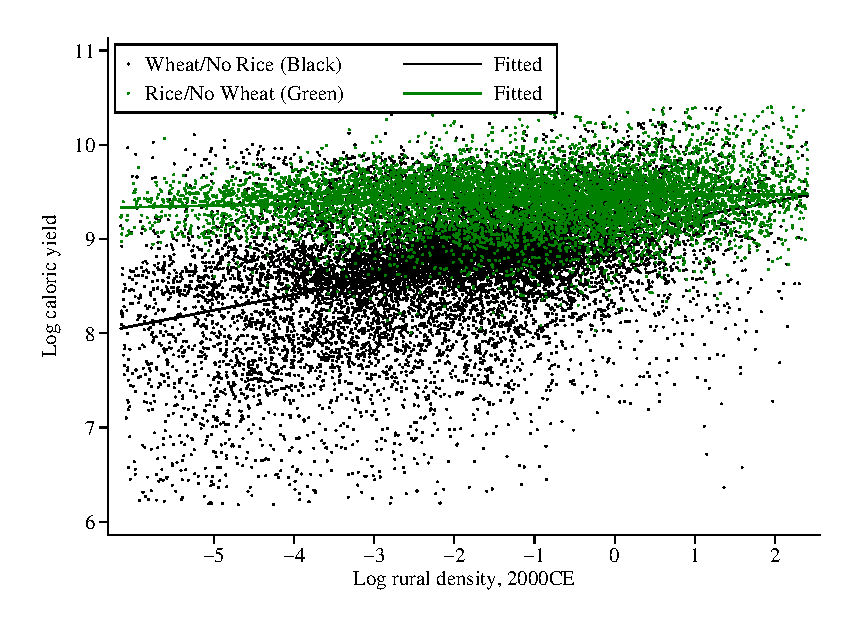
\includegraphics[width=1.0\textwidth]{fig_beta_crop.eps}
\end{center}
\vspace{-.5cm}\singlespacing {\footnotesize \textbf{Notes}: This figures shows the raw correlation of (log) caloric yield and (log) rural density for districts that are (a) suitable for wheat, but not for wet rice, and (b) suitable for wet rice but not for wheat. Rural population is from HYDE database \citep{hyde31}, and caloric yield is the author's calculations based on the data from \citet{galorozak2016}. The linear fits are from bivariate OLS regressions, without any fixed effects included. Based on equation (\ref{EQ_regress}), the slopes of these lines are estimates of $\beta$, the elasticity of agricultural output with respect to land.
}
\end{figure}


//////////////////////////////////////
// Create residual plot of baseline results
//////////////////////////////////////

qui reg ln_csi_yield urb_perc_2000 ln_light_mean i.state_id if dry_suit>0 & wet_suit==0, cluster(state_id)
predict csi_res_dry, res
qui reg ln_rurd_2000 urb_perc_2000 ln_light_mean i.state_id if dry_suit>0 & wet_suit==0, cluster(state_id)
predict rurd_res_dry, res

qui reg ln_csi_yield urb_perc_2000 ln_light_mean i.state_id if dry_suit==0 & wet_suit>0, cluster(state_id)
predict csi_res_wet, res
qui reg ln_rurd_2000 urb_perc_2000 ln_light_mean i.state_id if dry_suit==0 & wet_suit>0, cluster(state_id)
predict rurd_res_wet, res


scatter csi_res_dry rurd_res_dry if dry_suit>0 & wet_suit==0 & ln_csi_yield>0, msymbol(p) mcolor(black) ///
	|| lfit csi_res_dry rurd_res_dry if dry_suit>0 & wet_suit==0 & ln_csi_yield>0, clcolor(black) ///
	|| scatter csi_res_wet rurd_res_wet if dry_suit==0 & wet_suit>0, msymbol(p) mcolor(green) ///
	|| lfit csi_res_wet rurd_res_wet if dry_suit==0 & wet_suit>0, clcolor(green) ///
	xtitle("Residual log rural density, 2000CE") ytitle("Residual log caloric yield") ///
	ylabel(, angle(0) nogrid) graphregion(color(white)) /// xlabel(-5(1)2) ///
	legend(ring(0) pos(10) label(1 "Temperate (Black)") label(2 "Fitted") label(3 "Tropical (Green)") label(4 "Fitted"))
graph export "$output/fig_beta_crop.png", replace as(png)
graph export "$output/fig_beta_crop.eps", replace as(eps)

	


More broadly, HYDE's methodology of mapping of rural population may be driving our results. To assess this, we use a separate data source from the Global Rural-Urban Mapping Project (GRUMP), developed by \cite{Balketal2006}. This project also provides grid-cell level population counts, as well as ``urban masks'' that define cells within urban agglomerations. We extract the count of rural population in a given district from GRUMP as the count of population in all grid cells that are \textit{not} part of urban agglomerations. GRUMP's implicit rural population, then, will not necessarily conform to census reports of rural population (in principle, HYDE's count of rural population should conform). In the Appendix we show results using GRUMP's population data to measure rural density, and the results are consistent with the results from HYDE. There is one exception, which is that when we distinguish samples by their harvested area of crops, the estimated $\beta$ values are no longer statistically different between wheat and rice families. 

Combining this constraint with a positive relationship of living standards and population growth yields the canonical Malthusian model of stagnation \citep{ashraf2010dynamics}, and forms the basis for models of the transition from stagnation to sustained growth. The literature on the transition has grown large enough that it is difficult to provide a reasonable summary in a footnote. An overview of this unified growth literature can be found in \citet{Galor:2011uq}, who cites several key contributions \citep{gw00,galor2002natural,Hansen:2002fk,doepke2004accounting,cs2005,lagerlof2006,craftsmills2009,strulik2008population}. Explanations for the Great Divergence in income per capita are often framed in terms of these unified growth models \citep{kp2001,galor2008trading,vollrath2011,vv08,vv13,cs2015}. The Malthusian constraint features in quantitative work on contemporary developing countries that rely on agriculture \citep{Gollin:2007oq,Restuccia:2008hc,weilwilde2009,Gollin:2010ys,ev2016clim}, and is relevant for long-run growth in relatively rich countries due to possible limits to resources \citep{perettovalente2015}.